\documentclass[tikz,border=1pt,11pt]{standalone}
% Shared style for all diagrams. Text: Times; mathematics: Computer Modern, as in the paper.
% Figures are drawn at the paper's text width (432pt = 15.24cm), so sizes below are final.
\usepackage[T1]{fontenc}
\usepackage{times}
\usepackage{amsmath,amssymb}
\usepackage{pgfplots}
\usetikzlibrary{arrows.meta,calc,positioning,backgrounds,patterns,shapes.geometric}
\usepgfplotslibrary{groupplots,fillbetween}
\pgfplotsset{compat=1.18}
% Palette. Three identity hues (validated with the dataviz colour checks: lightness band,
% chroma floor, all-pairs CVD separation >= 8.9, normal-vision separation >= 18.5,
% contrast >= 3:1 on white) plus neutral inks and pale region fills.
\definecolor{ink}{HTML}{1D2733}      % text and exact reference curves
\definecolor{muted}{HTML}{56606B}    % secondary text
\definecolor{rule}{HTML}{8A929A}     % axes, guides
\definecolor{assess}{HTML}{1F6FA8}   % assessments; stable branches
\definecolor{process}{HTML}{1E9E73}  % accumulated processing
\definecolor{event}{HTML}{C5531F}    % completions, resets, driven paths
\definecolor{tolfill}{HTML}{E3EDF5}  % tolerance region
\definecolor{transfill}{HTML}{F2F4F6}% transition region
\definecolor{pausefill}{HTML}{E4F3EC}% processing paused
\tikzset{
 >={Stealth[length=2.1mm,width=1.5mm]},
 every picture/.append style={font=\small},
 lbl/.style={font=\small,text=ink,inner sep=1.5pt},
 note/.style={font=\footnotesize,text=muted,inner sep=1.5pt},
 paneltitle/.style={font=\small\bfseries,text=ink,inner sep=0pt},
 guide/.style={rule,line width=.45pt,densely dotted},
 report/.style={diamond,draw=ink,fill=white,line width=.8pt,inner sep=0pt,minimum size=5.2pt},
}
\pgfplotsset{
 every axis/.append style={
  axis lines*=left,
  axis line style={rule,line width=.5pt},
  tick style={rule,line width=.5pt},
  major tick length=2.2pt,
  tick align=outside,
  label style={font=\small,text=ink},
  tick label style={font=\small,text=ink},
  every axis plot/.append style={line width=1.15pt},
  scaled ticks=false,
  clip=false,
  xlabel style={inner sep=1pt},
  ylabel style={inner sep=1pt},
 },
}

\usetikzlibrary{decorations.pathreplacing}
% Figure 2. Episodes under a pausing clock with the capped reset R(u) = sgn(u) min(|u|, theta/2).
% A schematic, not a computation: the path is drawn by hand. Inside the tolerance band processing
% pauses; outside it processing accumulates (shaded) and the hazard rises, so a revision follows
% the exit with a delay. At a completion the assessment jumps to the reset level; the record keeps
% the date and the size of each jump, not the path or the processing behind it.
\begin{document}
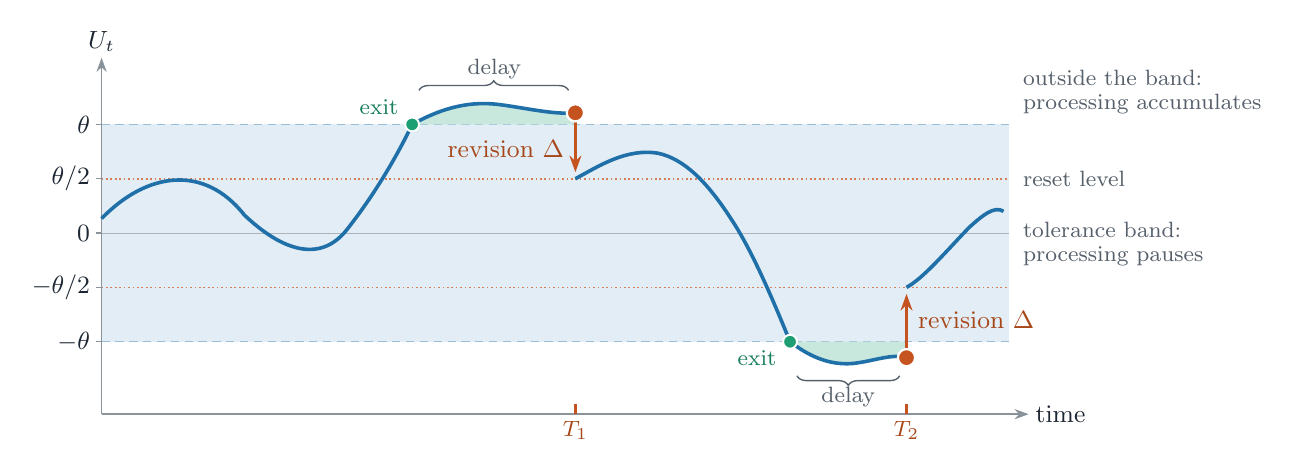
\begin{tikzpicture}[x=1.45cm,y=0.92cm]
\def\Th{1.5}      % tolerance band theta
\def\Tg{0.75}     % reset level theta/2
\def\Tend{7.95}
% ---- regions and reference lines -------------------------------------------------------
\fill[tolfill] (0,-\Th) rectangle (\Tend,\Th);
\draw[assess!45,line width=.4pt,densely dashed] (0,\Th) -- (\Tend,\Th);
\draw[assess!45,line width=.4pt,densely dashed] (0,-\Th) -- (\Tend,-\Th);
\draw[event!75,line width=.6pt,densely dotted] (0,\Tg) -- (\Tend,\Tg);
\draw[event!75,line width=.6pt,densely dotted] (0,-\Tg) -- (\Tend,-\Tg);
\draw[rule!70,line width=.4pt] (0,0) -- (\Tend,0);
% ---- axes -------------------------------------------------------------------------------
\draw[rule,line width=.5pt,-{Stealth[length=1.8mm,width=1.3mm]}] (0,-2.5) -- (0,2.42);
\draw[rule,line width=.5pt,-{Stealth[length=1.8mm,width=1.3mm]}] (0,-2.5) -- (8.12,-2.5);
\node[lbl,anchor=south] at (0,2.44) {$U_t$};
\node[lbl,anchor=west] at (8.14,-2.5) {time};
\foreach \y/\t in {1.5/{$\theta$},0.75/{$\theta/2$},0/{$0$},-0.75/{$-\theta/2$},-1.5/{$-\theta$}}{
  \draw[rule,line width=.5pt] (-0.045,\y) -- (0,\y);
  \node[lbl,anchor=east] at (-0.06,\y) {\t};
}
% ---- processing accumulates outside the band ---------------------------------------------
\fill[process!24]
  (2.72,1.50) .. controls (2.95,1.70) and (3.18,1.82) .. (3.45,1.78)
  .. controls (3.68,1.74) and (3.95,1.63) .. (4.15,1.66) -- (4.15,1.50) -- cycle;
\fill[process!24]
  (6.03,-1.50) .. controls (6.18,-1.68) and (6.36,-1.83) .. (6.58,-1.80)
  .. controls (6.76,-1.77) and (6.92,-1.66) .. (7.05,-1.72) -- (7.05,-1.50) -- cycle;
% ---- the assessment path, episode by episode ----------------------------------------------
\draw[assess,line width=1.3pt]
  (0,0.20) .. controls (0.40,0.85) and (0.90,0.95) .. (1.25,0.25)
  .. controls (1.55,-0.20) and (1.90,-0.45) .. (2.15,0.05)
  .. controls (2.40,0.55) and (2.60,1.10) .. (2.72,1.50)
  .. controls (2.95,1.70) and (3.18,1.82) .. (3.45,1.78)
  .. controls (3.68,1.74) and (3.95,1.63) .. (4.15,1.66);
\draw[assess,line width=1.3pt]
  (4.15,0.75) .. controls (4.35,0.92) and (4.60,1.18) .. (4.88,1.10)
  .. controls (5.10,1.02) and (5.30,0.72) .. (5.52,0.18)
  .. controls (5.70,-0.25) and (5.88,-0.92) .. (6.03,-1.50)
  .. controls (6.18,-1.68) and (6.36,-1.83) .. (6.58,-1.80)
  .. controls (6.76,-1.77) and (6.92,-1.66) .. (7.05,-1.72);
\draw[assess,line width=1.3pt]
  (7.05,-0.75) .. controls (7.20,-0.62) and (7.38,-0.28) .. (7.60,0.08)
  .. controls (7.72,0.25) and (7.82,0.38) .. (7.90,0.30);
% ---- exits from the band -----------------------------------------------------------------
\filldraw[fill=process,draw=white,line width=.7pt] (2.72,1.50) circle (2.5pt);
\filldraw[fill=process,draw=white,line width=.7pt] (6.03,-1.50) circle (2.5pt);
\node[note,text=process!80!black,anchor=east] at (2.64,1.74) {exit};
\node[note,text=process!80!black,anchor=east] at (5.95,-1.72) {exit};
% ---- completions and revisions -----------------------------------------------------------
\draw[event,line width=1.15pt,->] (4.15,1.60) -- (4.15,0.84);
\draw[event,line width=1.15pt,->] (7.05,-1.66) -- (7.05,-0.84);
\filldraw[fill=event,draw=white,line width=.8pt] (4.15,1.66) circle (3.1pt);
\filldraw[fill=event,draw=white,line width=.8pt] (7.05,-1.72) circle (3.1pt);
\node[lbl,text=event!85!black,anchor=east] at (4.09,1.16) {revision $\Delta$};
\node[lbl,text=event!85!black,anchor=west] at (7.11,-1.20) {revision $\Delta$};
% completion dates: what the record keeps, with the sizes of the jumps
\draw[event,line width=.8pt] (4.15,-2.5) -- (4.15,-2.36);
\draw[event,line width=.8pt] (7.05,-2.5) -- (7.05,-2.36);
\node[note,text=event!85!black,anchor=north] at (4.15,-2.54) {$T_1$};
\node[note,text=event!85!black,anchor=north] at (7.05,-2.54) {$T_2$};
% ---- delays between exit and completion --------------------------------------------------
\draw[decorate,decoration={brace,amplitude=3.5pt},muted,line width=.5pt] (2.78,1.97) -- (4.09,1.97);
\node[note,anchor=south] at (3.44,2.07) {delay};
\draw[decorate,decoration={brace,mirror,amplitude=3.5pt},muted,line width=.5pt] (6.09,-1.97) -- (6.99,-1.97);
\node[note,anchor=north] at (6.54,-2.06) {delay};
% ---- legend notes at the right -----------------------------------------------------------
\node[note,anchor=west,align=left] at (\Tend+0.08,1.95) {outside the band:\\[-1pt]processing accumulates};
\node[note,anchor=west,align=left] at (\Tend+0.08,0.75) {reset level};
\node[note,anchor=west,align=left] at (\Tend+0.08,-0.15) {tolerance band:\\[-1pt]processing pauses};
\end{tikzpicture}
\end{document}
